\chapter{Curved mesh generation}
\section{Introduction}

The problem of curved mesh generation involves at least one issue - the placement of the boundary ``high-order" nodes. A description of a high-order boundary is required, and the optimal placement of high-order boundary nodes must be decided.

Additionally, we usually need to deal with one more issue - maintaining the quality of elements near the boundary after placing the high-order boundary nodes. The deformation of the initially polygonal/polyhedral boundary to get a curved boundary usually causes the quality of boundary elements to get reduced. In cases with a viscous mesh, these elements may even become invalid \cite{curve:persson, gmsh:untangling}. Thus, the deformation of the boundary must be propagated into the domain, to displace interior nodes upto at least some distance from the boundary.

In our knowledge, there are, broadly speaking, three types of methods to achieve movement of the interior nodes. The first type uses models based on solid mechanics to try to achieve valid mesh movement, as explained in the previous chapter. The second type of technique to move the interior nodes involves interpolation of the boundary displacement to interior nodes, again, as previously explained. Finally, researchers have ``untangled" the near-boundary elements, and otherwise improved the quality of the mesh, by optimization processes. The cost function is usually some kind of curved-mesh quality measure. One prominent example of this is in the Gmsh meshing software \cite{gmsh:untangling}. One interesting development in curved mesh generation is due to Ims at. al. \cite{curve:meshcurve}, in which explicit interpolation (\cite{mm:explicit}) is used to curve the interior of the mesh. 

We present an alternative approach based on radial basis functions. This approach is compared to the more prevalent methods of linear elasticity \cite{curve:hartmann}.

In the rest of the sections, we discuss the methodology used to generate 2D unstructured quadratic meshes from linear meshes, and then present examples to demonstrate the effectiveness of our method. We compare the quality of meshes given by the RBF interpolation method and the linear-elasticity method.

\section{Method}

We initially preprocess the linear mesh to generate a straight-faceted high-order mesh. To do this, we introduce extra nodes along edges, in faces and inside cells as required. Next, we either use CAD data or use a high-order boundary reconstruction method to obtain the actual positions of boundary high-order nodes. Finally, interior nodes are moved according to the boundary displacement imposed because of the previous step.

\subsection{Spline reconstruction for boundaries of 2D meshes}
Since only the linear mesh is taken as input, a high-order boundary representation first needs to be reconstructed from the piecewise linear $C^0$ boundary. For 2D meshes, we use a cubic spline reconstruction to get a smooth ($C^2$) parametric curve describing the boundary. All boundary nodes are used as spline control points, and we get a cubic function between every two consecutive boundary nodes. At the control points, we require the two spline curves meeting there to share a common tangent and curvature, thus enforcing $C^2$ continuity. Since it is common for the true boundary to be specified in terms of cubic spline curves, this is expected to give us an accurate reconstruction. Corners are detected by comparing the normal vectors of the two facets sharing a point. If the dot product between the two normal vectors is below a particular user-specified threshold, the point is considered as a corner and is not smoothed over by the reconstruction procedure. Alternatively, the user can list all the corner points as input. The spline reconstruction requires the solution of a symmetric positive definite linear system, of size equal to the number of boundary nodes in the curved part of the boundary, in order to calculate the cubic spline coefficients. The system(s) can be solved quickly using a conjugate gradient (CG) solver. More details are given in appendix \ref{app:spline}.

Instead of a global reconstruction by cubic splines, we could also use a local reconstruction at each boundary node. This is described more generally for 3D meshes in the next section.

Once we have the smooth reconstructed boundary, we calculate the final positions of the boundary nodes in the curved mesh. This is currently done by simply moving the high-order boundary nodes, originally at regular intervals on the boundary facet, to corresponding intervals in parameter space on the cubic spline curve associated with that facet. This method is found to be quite robust for the meshes tested. Thus, the boundary displacements are obtained. Alternatively, if the CAD geometry is available, the displacements can be computed using it.

\subsection{Surface reconstruction in the general case}
For some meshes, the requirement of global $C^2$ continuity is too restrictive. Also, a procedure similar to that described in the previous section would be quite expensive for surfaces in $\mathbb{R}^3$. We therefore consider local fittings of 2D Taylor polynomials at every boundary vertex, as described in \cite{sr:jiaowang} as ``Weighted Averaging of Local Fittings" (WALF). In their paper, Jiao and Wang fit local 2D Taylor polynomials to each vertex of the surface mesh. The coefficients, that is, the derivatives of a local height function in a local coordinate system centered at the vertex, are solved for using vertex position data from a neighborhood of that vertex. It is ensured that there are more neighboring points being considered for data than the number of unknowns to solve for, thereby obtaining an over-determined system of equations. This is solved by a weighted least-squares approach. We adopt a variation of this approach, as suggested by Ims et. al. \cite{curve:meshcurve}, in that local Taylor polynomials are fitted to every face-center, for reasons elaborated below. We first describe the original method in \cite{sr:jiaowang}.

In Jiao and Wang's method, a local $uvw$ coordinate system is determined at each vertex of the surface mesh. How this is done is suggested in \cite{sr:diffquant} by Jiao and Zha. An estimate of the outward normal to the surface at the vertex serves as the $w$-axis of the local coordinate frame. In our work, the normal is estimated as a weighted average of the face-normals of the faces surrounding the vertex. We use either an inverse-distance weighted average or an area-weighted average. Once the normal direction $\hat{\bld{n}}$ is decided, the $u$ direction is taken as any direction normal to the $w$-axis. Let the $u$ direction be along $\bld{t}_1$ in global coordinates. Finally, $\hat{\bld{t}_2} = \hat{\bld{n}} \times \hat{\bld{t}_1}$ forms the $v$ direction. Thus we obtain a right-handed $uvw$ coordinate system. We can transform any point with global coordinates $\bld{x}$ can be transformed to $\bld{u}$ in the local frame of the point at $\bld{x}_0$ as
\begin{equation}
\bld{u} = \bld{Q} (\bld{x} - \bld{x}_0)
\end{equation}
where
\begin{equation}
\bld{Q} =
\begin{bmatrix}
\hat{\bld{t}_1} & \vert & \hat{\bld{t}_2} & \vert & \hat{\bld{n}}
\end{bmatrix}
\end{equation}
is an orthogonal rotation matrix.

Next, a locally high-order surface is reconstructed by expanding a local height function in a Taylor polynomial around that vertex. For reconsucting a $d$-degree surface, the local height function $h$ is expressed as
\begin{equation}
h(u,v) \approx \sum_{i=0}^d \sum_{j\geq 0,k\geq 0}^{j+k \leq d} \frac{u^j v^k}{j!k!} D_{jk}
\end{equation}
where $D_{jk} := \frac{\partial^{j+k} h}{\partial^j u \, \partial^k v}$,
Suppose we consider $m$ linear mesh vertices around a vertex for the reconstruction at the latter vertex, we obtain a system of equations to solve for the derivatives $D_{jk}$. Thus we have an $m \times n$ system with $n:= \frac12 (d+1)(d+2)$, i.e.,
\begin{equation}
\sum_{i=0}^d \sum_{j\geq 0,k\geq 0}^{j+k \leq d} \frac{u_p^j v_p^k}{j!k!} D_{jk} \approx h_p
\label{eq:sr_taylorequation}
\end{equation}
for $p \in \{1,2,...,m \}$. If $m \ge n$, this system can be solved in a least-squares sense. We can write the system of equations as
\begin{equation}
\bld{V} \bld{D} = \bld{f}
\end{equation}
where $\bld{V} (m\times n)$ is the generalized Vandermonde matrix for 2D Taylor polynomials, $\bld{D}$ is the $n$-vector of derivatives of the height function at the local origin, and $\bld{f}$ is the $m$-vector of heights of points in the reconstruction stencil. The system is solved by a weighted least-squares method. This is done for each vertex on the boundary.

For each vertex, the reconstruction stencil is selected according to the degree of polynomial surface required. It is claimed \cite{sr:diffquant} that $m$ should be from 1.5 to 2 times $n$. A general method for selecting reconstruction stencils for triangular and rectangular surface meshes is given by Jiao and Wang \cite{sr:jiaowang}. Here, we are mainly concerned with obtaining good P2 discretizations, for which the stencil is shown in figure \ref{f:stencil}. All vertices shown are used in reconstructing the surface at the center vertex.

\begin{figure}
	\centering
	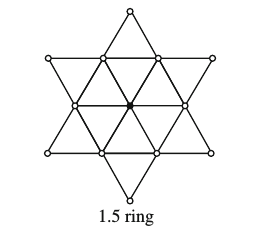
\includegraphics[scale=1.0]{stencil}
	\caption{Stencil for reconstruction of P2 surface; from \cite{sr:jiaowang}}
	\label{f:stencil}
\end{figure}

The weighted least-squares problem is expressed as
\begin{equation}
\min_{\bld{D}} \lVert \bld{W}(\bld{V}\bld{D}-\bld{f})\rVert_2
\label{eq:sr_wls}
\end{equation}
where $\bld{W}$ is an $m \times m$ diagonal weighting matrix. The weight for the $i$th point in the stencil is taken as (see \cite{sr:diffquant})
\begin{eqnarray}
w_i &=& \frac{\gamma_i^+}{(\sqrt{\lVert\bld{u}_i\rVert^2 + \epsilon})^{d/2}} \, , \text{where} \\
\gamma_i^+ &=& \max\{0,\hat{\bld{n}_i}^ T\hat{\bld{n}_0}\}, \\
\epsilon &=& \frac{1}{100m} \sum_{i=1}^m \lVert\bld{u}_i \rVert^2.
\label{eq:sr_weight}
\end{eqnarray}
In the above equations, $\bld{u}_i$ and $\hat{\bld{n}_i}$ denote the position of and normal at the $i$ vertex in the reconstruction stencil, respectively, while $\hat{\bld{n}_0}$ denotes the normal at the vertex for which the local reconstruction is being computed.

The least-squares problem is solved by a QR factorization method using Householder transformations. Once the coefficients $\bld{D}$ are found for each point, we can move the high-order nodes accordingly.

\subsection{Interior mesh movement}

To propagate the boundary motion to the interior of the mesh, we favor interpolation by radial basis functions (RBFs) \cite{mm:rbf}. We have also used linear elasticity to propagate the mesh movement to the interior. The isotropic linear elasticity variational formulation, as given by Gockenbach \cite{gockenbach}, is implemented in a P2 Galerkin FEM code for generation of quadratic meshes. In this case however, the size of the linear system to be solved is proportional to the total number of nodes in the mesh.

Though the RBF method requires the solution of a linear system of size proportional to only the number of boundary points, extra computation is required to evaluate equation \eqref{eqn:rbf} at each of the interior nodes to compute their displacements. In comparison, elasticity-based methods directly give us the displacements.

Several variants of the Delaunay graph mapping method were also attempted for generating curved meshes.

********* TODO: DESCRIBE WHY DGM AND DG-RBF FAIL FOR CURVED MESH GENERATION. DESCRIBE THE 2-STEP RBF-DG METHOD, AND WHY THAT DOES NOT WORK EITHER *********


